
\documentclass{article}

\usepackage{amsmath}
\usepackage{amssymb}
\usepackage{bbm}
\usepackage{comment}
\usepackage{enumerate}

\usepackage{extramarks} % Required for headers and footers
\usepackage{fancyhdr}

\usepackage{graphicx} % Required to insert images
\usepackage{verbatim}


% Margins
\topmargin=-0.45in
\evensidemargin=0in
\oddsidemargin=0in
\textwidth=6.5in
\textheight=9.0in
\headsep=0.25in 

\linespread{1.1} % Line spacing

% Set up the header and footer
\pagestyle{fancy}
\lhead{Linear Algebra with Application\\
to Engineering Computation}
\chead{}
\rhead{CME 200/ME300A\\
M. Gerritsen\\
Fall 2013}
\headheight = 40pt

\renewcommand\headrulewidth{0.4pt} % Size of the header rule
\renewcommand\footrulewidth{0.4pt} % Size of the footer rule

\setlength\parindent{0pt} % Removes all indentation from paragraphs

%Add useful short-cut commands here

%math symbols such as R, and Pr
\newcommand{\I}{\ensuremath{\operatorname{I}}}
\newcommand{\One}[1]{\ensuremath{\mathbbm{1}_{\left \{ #1 \right \}}}}
\newcommand{\E}{\ensuremath{\mathbb{E}}}
\newcommand{\R}{\ensuremath{\mathbb{R}}}
\newcommand{\N}{\ensuremath{\mathbb{N}}}


%1st order derivative wrt x
\newcommand{\dxone}[1]{\frac{d#1}{dx}}
%2nd order derivative wrt x
\newcommand{\dxtwo}[1]{\frac{d^2#1}{dx^2}}
%th in the exponent (e.g. when writing ith, instead use i$\eth$)
\newcommand{\tth}{^{\text{th}}}

%short-cuts for Greek letters
\newcommand{\al}{\alpha}
\newcommand{\dlt}{\delta}
\newcommand{\eps}{\epsilon}
\newcommand{\la}{\lambda}


%norms
\newcommand{\norm}[1]{\|#1\|}
\newcommand{\normII}[1]{\|#1\|_2}

\newcommand{\x}{\times}
%inverse
\newcommand{\inv}{^{-1}}
%cond
\newcommand{\cond}{\mathrm{cond}}
%trace
\newcommand{\trace}{\mathrm{trace}}
\newcommand{\tr}{\mathrm{tr}}
%rank
\newcommand{\rank}{\mathrm{rank}}

 
%matrices
\newcommand{\bmat}[1]{\begin{bmatrix}#1\end{bmatrix}} 
\newcommand{\pmat}[1]{\begin{pmatrix}#1\end{pmatrix}} 
 

%parentheses
\newcommand{\paren}[1]{\left(#1\right)}
\newcommand{\brac}[1]{\left[#1\right]}
\newcommand{\cbrac}[1]{\left\{#1\right\}} 


\newcommand{\twith}{\text{ with }}
\newcommand{\tand}{\text{ and }}
\newcommand{\tfor}{\text{ for }}
\newcommand{\tor}{\text{ or }}
\newcommand{\tat}{\text{ at }}

\newcommand{\ip}{_{i+1}}
\newcommand{\im}{_{i-1}}

\newcommand{\half}{\frac{1}{2}}
\newcommand{\oneby}[1]{\frac{1}{#1}}
\newcommand{\overto}[1]{\overset{#1}{\longrightarrow}}
%----------------------------------------------------------------------------------------
%       DOCUMENT STRUCTURE COMMANDS
%       Skip this unless you know what you're doing
%----------------------------------------------------------------------------------------

% Header and footer for when a page split occurs within a problem environment
\newcommand{\enterProblemHeader}[1]{
\nobreak\extramarks{#1}{#1 continued on next page\ldots}\nobreak
\nobreak\extramarks{#1 (continued)}{#1 continued on next page\ldots}\nobreak
}

% Header and footer for when a page split occurs between problem environments
\newcommand{\exitProblemHeader}[1]{
\nobreak\extramarks{#1 (continued)}{#1 continued on next page\ldots}\nobreak
\nobreak\extramarks{#1}{}\nobreak
}

\setcounter{secnumdepth}{0} % Removes default section numbers
\newcounter{homeworkProblemCounter} % Creates a counter to keep track of the number of problems

\newcommand{\homeworkProblemName}{}
\newenvironment{homeworkProblem}[1][Problem \arabic{homeworkProblemCounter}]{ % Makes a new environment called homeworkProblem which takes 1 argument (custom name) but the default is "Problem #"
\stepcounter{homeworkProblemCounter} % Increase counter for number of problems
\renewcommand{\homeworkProblemName}{#1} % Assign \homeworkProblemName the name of the problem
\section{\homeworkProblemName} % Make a section in the document with the custom problem count
\enterProblemHeader{\homeworkProblemName} % Header and footer within the environment
}{
\exitProblemHeader{\homeworkProblemName} % Header and footer after the environment
}
\newcommand\overmat[2]{%
  \makebox[0pt][l]{$\smash{\overbrace{\phantom{%
    \begin{matrix}#2\end{matrix}}}^{\text{$#1$}}}$}#2}

\newcommand{\problemAnswer}[1]{ % Defines the problem answer command with the content as the only argument
\noindent\framebox[\columnwidth][c]{\begin{minipage}{0.98\columnwidth}#1\end{minipage}} % Makes the box around the problem answer and puts the content inside
}

\title{Assignment 7 - Solutions}
\date{Issued: November 13, 2013}
\author{Due: November 20, in class\\
No late assignments accepted}

%----------------------------------------------------------------------------------------

\begin{document}

\maketitle
\thispagestyle{fancy}

% Problem 1
\begin{homeworkProblem}
\begin{enumerate}[(a)]

\item Let $A$ be an $n \x n$ symmetric matrix.
Let $\vec q_i$ and $\vec q_j$ be the eigenvectors of $A$ corresponding to the eigenvalues $\la_i$ and $\la_j$ respectively. Show that if $\la_i \ne \la_j$, then $\vec q_i$ and $\vec q_j$ are orthogonal.

\item Let $A$ be an $n \x n$ matrix. We say that $A$ is {\bf positive definite} if for any non-zero vector $\vec x$, the following inequality holds
\[ \vec x^T A \vec x > 0. \]
Show that the eigenvalues of a positive definite matrix $A$ are all positive.

\item Let $A$ be an $n \x n$ matrix. Show that 
\[ \tr(A) = \sum_{i=1}^n \la_i, \] 
where $\la_1, \dots, \la_n$ are the eigenvalues of $A$ ($\la_i$'s do not have to be all different). You may assume that all eigenvalues of $A$ are real numbers.

[Hint 1: One way to prove this is to use the fact that any square matrix with real eigenvalues can be decomposed in the following way (called Schur decomposition)
\[A = QRQ^T,\]
where $R$ is an upper triangular matrix and $Q$ is an orthogonal matrix. 

Hint 2: You might find it useful to recall the properties of trace.]
\end{enumerate}
\end{homeworkProblem}

{\bf Solution:}

\begin{enumerate}[(a)]
\item By the definition of eigenvalues/eigenvectors, we have
\[ A\vec q_i = \la_i \vec q_i, \quad A\vec q_j = \la_j \vec q_j \]
Then, since $A = A^T$, 
\[ \la_i \vec q_j^T \vec q_i = \vec q_j^T \la_i \vec q_i = \vec q_j^T A \vec q_i = \vec q_j^T A^T \vec q_i = (A \vec q_j)^T \vec q_i = (\la_j \vec q_j)^T \vec q_i = \la_j \vec q_j^T \vec q_i. \]
Rearranging, we have
\[ (\la_i - \la_j) \vec q_j^T \vec q_i = 0. \]
When $\la_i \ne \la_j$ the term in the parentheses is non-zero, so it follows that
\[ \vec q_j^T \vec q_i = 0, \]
which means that $\vec q_i$ and $\vec q_j$ are orthogonal.

\item Let $\la$ be an eigenvalue of $A$ corresponding to an eigenvector $\vec q$, i.e.
\[ A\vec q = \la \vec q. \]
Then, since $A$ is positive definite, we have
\[ 0 < \vec q^T A \vec q = \vec q^T \la \vec q = \la \normII{\vec q}^2. \]
Since $\normII{\vec q} > 0$ ($\vec q \ne \vec 0$ for any eigenvector $\vec q$), it follows that $\la>0$.

\item Consider the Schur decomposition of $A$,
\[ A = QRQ^T. \]
Using the property of trace that $\tr(ABC) = \tr(BCA) = \tr(CAB)$ (invariance under cyclic permutations), we have
\[ \tr(A) = \tr(QRQ^T) = \tr(RQ^TQ) = \tr(R) = \sum_{i=1}^n R_{ii}. \]
We now prove that for any (upper) triangular matrix $R$ the diagonal elements of $R$ are its eigenvalues. Consider the characteristic polynomial of $R$,
\[ p(\la) = \det(\la I - R) = (\la-R_{11})(\la-R_{22})\cdots(\la-R_{nn}) = \prod_{i=1}^n (\la-R_{ii}), \]
where for the second equality we used the fact that the determinant of a triangular matrix is the product of its diagonal entries.
Since the roots of a characteristic equation are the eigenvalues of $R$, we can immediately see that $\la_i = R_{ii}\tfor i=1,\dots, n$, so that
\[ \tr(A) = \sum_{i=1}^n R_{ii} = \sum_{i=1}^n \la_i. \]
Now, it remains to show that the eigenvalues of $R$ are equal to the eigenvalues of $A$.
If $\al$ is an eigenvalue of $A$ corresponding to eigenvector $\vec v$, then
\[ \al \vec v = A \vec v = QRQ^T \vec v. \]
Pre-multiplying by $Q^T$, we have
\[ Q^T \al \vec v = RQ^T \vec v, \]
\[ \al Q^T \vec v = RQ^T \vec v, \]
\[ \al \vec u = R \vec u, \]
where $\vec u = Q^T \vec v$ is an eigenvector of $R$ corresponding to eigenvalue $\al$. This proves the claim. Therefore,
\[ \tr(A) = \sum_{i=1}^n \la_i, \]
where $\la_i,\ i=1,\dots, n$ are the eigenvalues of $A$ (and $R$).

[{\bf Note.} The fact that eigenvalues of $A$ and $R$ were the same holds in a more general setting. We say that two matrices $A$ and $B$ are {\bf similar} if there exists and invertible matrix $P$, such that 
\[ B = P\inv A P. \]
The prove above shows that all similar matrices $A$ and $B$ have the same set of eigenvalues. This property is referred to as the {\bf invariance of eigenvalues under similarity transformations}.]
\end{enumerate}


\begin{homeworkProblem} %(15)

We are interested in finding the fixed points (the points at which the time derivatives are zero) of the following system of equations:
\begin{align*}
\frac{dx_1}{dt} &= x_1(a-bx_2)\\
\frac{dx_2}{dt} &= -x_2(c-dx_1)
\end{align*}
for $a = 3, b = 1, c = 2, d = 1$. We can use the Newton-Raphson method to find these fixed points, simply by setting the derivatives zero in the given system of equations. 
\begin{enumerate}[(a)]
\item
In the scalar case, Newton-Raphson breaks down at points at which the derivative of the nonlinear function is zero. In general, where can it break down for systems of nonlinear equations? For the system given above, find the troublesome points.
\item
Find the fixed points of the above system analytically. 
\item
Find all fixed points using repeated application of the Newton-Raphson method. You will have to judiciously choose your starting points (but of course, you are not allowed to use the known roots as starting points!). You may use MATLAB to program the method if you like. 
\end{enumerate}
{\bf Solution:}
\begin{enumerate}
\item
The Newton-Raphson method can break down for systems of nonlinear equations when the Jacobian matrix is singular. Let’s examine the given system:
\begin{align*}
f_1(x_1,x_2) &= x_1(3-x_2)\\
f_2(x_1,x_2) &= -x_2(2-x_1)\\
J(x_1,x_2) &= \pmat{\frac{\partial f_1}{\partial x_1} & \frac{\partial f_1}{\partial x_2}\\\frac{\partial f_2}{\partial x_1} & \frac{\partial f_2}{\partial x_2}} \\
&= \pmat{3-x_2 & -x_1 \\ x_2 & x_1 - 2}
\end{align*}
The troublesome points can be found by setting the determinant of $J=0$
\begin{align*}
\det(J) &= (3-x_2)(x_1-2)+x_1x_2\\
&= 0\\
3x_1+2x_2 &= 0
\end{align*}
Hence, the troublesome points in this case form a line in two dimensional space.
\item
The fixed points of the above system occur when the derivatives of $x$ w.r.t. $t$ are zero. Therefore
\begin{align*}
f_1(x_1,x_2) &= x_1(3-x_2) = 0\\
f_2(x_1,x_2) &= -x_2(2-x_1) = 0\\
\end{align*}
This is easily solved to be (0,0) and (2,3).
\item
The equation to solve at every iteration is
\begin{align*}
J(\vec{x}^{(k)})(\vec{x}^{(k+1)}-\vec{x}^{(k)}) 
= -f(\vec{x}^{(k)})
\end{align*}
\begin{align*}
\pmat{{x_1}^{(k+1)}\\ {x_2}^{(k+1)}} = -\pmat{3-{x_2}^{(k)}  & {x_1}^{(k)}\\{x_2}^{(k)} & {x_1}^{(k)} - 2}^{-1}\pmat{x_1^{(k)}(3-x_2^{(k)}) \\ x_2^{(k)}(2-x_1^{(k)})} + \pmat{x_1^{(k)} \\x_2^{(k)}}
\end{align*}
This iteration can be computed in Matlab or by hand. Of course, we should not come across points that make the Jacobian singular and therefore, we choose the starting points to be not close to the line of troublesome points calculated in the first part. Interestingly, travelling across the line when choosing the starting point, changes the final solution. So, we choose one starting point which lies above the line(e.g. (4,2)) to get (2,3) and another which is below the line(e.g (-1,1)) to get the other solution(0,0). This takes about 5 iterations to converge.
\begin{align*}
\vec{x}^{(1)} = \pmat{4\\2} \rightarrow 
\vec{x}^{(2)} = \pmat{1.6\\2.4} \rightarrow 
\vec{x}^{(3)} = \pmat{2.1333\\3.2}\rightarrow 
\vec{x}^{(4)} = \pmat{2.0078\\3.2}\rightarrow 
\vec{x}^{(5)} = \pmat{2\\3}
\end{align*}
\begin{align*}
\vec{x}^{(1)} = \pmat{-1\\1} \rightarrow 
\vec{x}^{(2)} = \pmat{0.2857\\0.4286} \rightarrow 
\vec{x}^{(3)} = \pmat{-0.0015\\-0.0023}\rightarrow 
\vec{x}^{(4)} = 10^{-5}\pmat{0.1191\\0.1786}\rightarrow 
\vec{x}^{(5)} = 10^{-11}\pmat{-0.0709\\-0.1063}
\end{align*}

\end{enumerate}
\end{homeworkProblem}



% Problem 2
\begin{homeworkProblem} %(15)

\begin{enumerate}[(a)]
\item Find the best straight-line fit to the following measurements, and graph your solution:
\begin{align*}
y_1 = 2 \tat t_1 = -1,\quad\quad 	&y_2 = 0 \tat t_2 = 0,\\ 
y_3 = -3 \tat t_3 = 1,\quad\quad 	&y_4= -5 \tat t_4 = 2.
\end{align*}
What is the norm of the residual?

\item Suppose that instead of a straight line, we fit the data above by the parabolic function:
\[ y_i = a_2 x_i^2 + a_1x_i + a_0. \]
Derive the over-determined system $A\vec x=\vec b$ to which least squares could be applied to find this quadratic fit.

\item Let's look at the general problem of making $n$ observations $y_i,\ i=1,2,\dots,n$ at $n$ different times $t_i$. You can extend what you did in the last two parts to find polynomial fits of degree $k$ ($y_i = a_kt_i^k + a_{k-1}t_i^{k-1} + \dots + a_1t_i + a_0$) by using least squares. If $k<n-1$, what
would the over-determined system $A\vec x = \vec b$ look like for this general case?

\item Prove that for $k=n-1$, the system $A\vec x = \vec b$ will no longer be over-determined and we can find a unique fit by solving $A\vec x = \vec b$ instead of the normal equations.

\item Consider the systems you solved for in part c and d. For $0<k<n$, how does the norm of the residual change as we increase $k$?
\end{enumerate}
\end{homeworkProblem}

{\bf Solution:}
\begin{enumerate}[(a)]
\item We want to solve the following over-determined system of equations $A\vec x = \vec b$:
\[ \pmat{t_1 & 1\\
		t_2 & 1\\
		t_3 & 1\\
		t_4 & 1 }
   \pmat{a_1 \\ a_0} =
   \pmat{y_1\\ y_2\\ y_3\\ y_4}. \]
This leads us to the normal equation $A^TA\vec x = A^T \vec b$. That is:
\[ \pmat{t_1 & t_2 & t_3 & t_4\\ 1 & 1 & 1 & 1}
   \pmat{t_1 & 1\\
		t_2 & 1\\
		t_3 & 1\\
		t_4 & 1 }
   \pmat{a_1 \\ a_0} =
   \pmat{\sum\limits_{i=1}^4 t_i^2 & \sum\limits_{i=1}^4 t_i\\
		\sum\limits_{i=1}^4 t_i & \sum\limits_{i=1}^4 1 }
   \pmat{a_1 \\ a_0} = 
   \pmat{\sum\limits_{i=1}^4 t_i y_i\\ \sum\limits_{i=1}^4 y_i } \to \]
\[ \to \pmat{6 & 2 \\ 2 & 4 } \pmat{a_1\\ a_0 } = \pmat{-15\\ -6} \to    
   \pmat{a_1\\ a_0 } = \pmat{-2.4\\ -0.3} . \]
So the best fit line is $y= -2.4 t - 0.3$. The graph is shown in Figure~\ref{fig:pb1a}.
\begin{figure}[ht!]
\centering
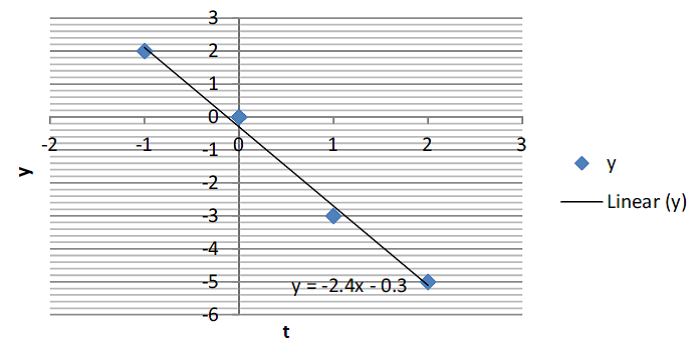
\includegraphics[width=.8\linewidth]{pb1a.png}
\caption{1(a) Best fit line.}
\label{fig:pb1a}
\end{figure}
The norm of the residual is given by $\normII{\vec b-A\vec x}$:
\[ \vec b-A\vec x =
  \pmat{y_1\\ y_2\\ y_3\\ y_4} - 
  \pmat{t_1 & 1\\
		t_2 & 1\\
		t_3 & 1\\
		t_4 & 1 }
  \pmat{a_1 \\ a_0} \to
  \pmat{2\\ 0\\ -3\\ -5} - 
  \pmat{-1 & 1\\
		0 & 1\\
		1 & 1\\
		2 & 1 }
   \pmat{-2.4 \\ -0.3} =
  \pmat{-0.1 \\ 0.3 \\ -0.3 \\ 0.1} \to \normII{\vec b-A\vec x} = 0.4472. \]
\newpage
\item In this case $A\vec x = \vec b$ is:
\[ \pmat{t_1^2 & t_1 & 1\\
		t_2^2 & t_2 & 1\\
		t_3^2 & t_3 & 1\\
		t_4^2 & t_4 & 1 }
   \pmat{a_2 \\ a_1 \\ a_0} =
   \pmat{y_1\\ y_2\\ y_3\\ y_4}, \text{ which is } \]

\[ \pmat{1 & -1 & 1\\
		0 & 0 & 1\\
		1 & 1 & 1\\
		4 & 2 & 1 }
   \pmat{a_2 \\ a_1 \\ a_0} =
   \pmat{2\\ 0\\ -3\\ -5}. \]
   
\item In the general case the over-determined system would like this:
\[ \pmat{t_1^k & t_1^{k-1} & \dots & 1\\
		t_2^k & t_2^{k-1} & \dots & 1\\
		\vdots & \vdots & \ddots & \vdots \\
		t_n^k & t_n^{k-1} & \dots & 1 }
   \pmat{a_k \\ a_{k-1} \\ \vdots \\ a_0} =
   \pmat{y_1\\ y_2\\ \vdots \\ y_n}. \]

\item In the case when $k = n-1$, we want to solve the equation $A\vec x = \vec b$:
\[ \pmat{t_1^{n-1} & t_1^{n-2} & \dots & 1\\
		t_2^{n-1} & t_2^{n-2} & \dots & 1\\
		\vdots & \vdots & \ddots & \vdots \\
		t_n^{n-1} & t_n^{n-2} & \dots & 1 }
   \pmat{a_{n-1} \\ a_{n-2} \\ \vdots \\ a_0} =
   \pmat{y_1\\ y_2\\ \vdots \\ y_n}, \]
where $A$ is an $n \x n$ matrix. We need to prove that $A$ is non-singular in order to show that a solution to this equation exists and is unique. We will examine the null space of $A$. Let's assume that $A \vec x = \vec 0$ has a solution,
\[  \vec x = \pmat{a_{n-1}'\\ a_{n-2}' \\ \vdots \\ a_{0}'}. \]
Then the polynomial $p(t) = a_{n-1}'t^{n-1} + a_{n-2}'t^{n-2} + \dots + a_{1}'t + a_{0}'$ has $n$ distinct roots, $t_1, t_2, \dots, t_n$. However, the fundamental theorem of algebra states that a non-zero polynomial of degree $n$ can at most have $n-1$ real roots (for example a quadratic function has at most two roots). Therefore, since $p(t)$ can have at most $n-1$ distinct roots, we must have $\vec x = \vec 0$. Thus, the nullspace consists of only the zero vector; hence, $r=n$ and the matrix $A$ is full-rank and nonsingular.

\item If we take the norm of the residual for $k$ to be $e_k = \norm{A_k \vec x - \vec b}$, then:
\[ e_1 \ge e_2 \ge \dots \ge e_{n-1} = 0. \]
To prove this, let's assume the contrary, i.e. for $i<j,\ e_i < e_j$ then:
\[ e_i = \normII{a_{i}\vec t_{i} + a_{i-1}\vec t_{i-1} + \dots + a_{1}\vec t_1 + a_{0}\vec t_0 - \vec b} < \normII{a'_{j}\vec t_{j} + a'_{j-1}\vec t_{j-1} + \dots + a'_{i}\vec t_{i} + \dots + a'_{1}\vec t_1 + a'_{0}\vec t_0 - \vec b} = e_j, \]
where $\vec t_k = \bmat{t_1^k & t_2^k & \dots & t_n^k}^T$. Since the normal equation minimizes the norm of the residual, we know that $a'_j, a'_{j-1},\dots a'_i,\dots,a'_1,a'_0$ are computed such that $e_j$ is minimized. However, setting $a'_j = a'_{j-1} = \dots = a'_{i+1} = 0$ and $a'_k = a_k$ for $k<i+1$, we see that this results in a smaller norm so we have a contradiction and our assumption is invalid. Thus, the norm cannot increase as we increase $k$. The fact that $e_{n-1} = 0$ is quite obvious from the last part where it was shown that $\vec x$ can be found from solving $A \vec x = \vec b$.


\end{enumerate}


% Problem 3
\begin{homeworkProblem}
\begin{enumerate}[(a)]
\item
From class we know that $P=A(A^TA)^{-1}A^T$ is an orthogonal projection matrix that projects onto the column space of $A$. Prove that $P$ is symmetric and $P^2= P^TP = P$. 
\item[(b)*]
In general, a matrix which satisfies $P^2=P$ is a projector. Show that if a projector matrix is symmetric, then it is an orthogonal projector.
\item[(c)]
Show that regardless of the rank of $A$, the equation $A^TAx=A^T
b$ always has at least one solution. 
\end{enumerate}

{\bf Solution:}

\begin{enumerate}[(a)]
\item
\begin{align*}
P^T &= (A(A^TA)^{-1}A^T)^T\\
&=(A^T)^T((A^TA)^{-1})^TA^T \\
&= A((A^TA)^T)^{-1}A^T \\
&= A(A^TA)^{-1}A^T\\
&= P
\end{align*}
Therefore $P$ is symmetric. Also
\begin{align*}
P^2 &= PP \\
&= P^TP \\
&= A(A^TA)^{-1}A^TA(A^TA)^{-1}A^T \\
&= A(A^TA)^{-1}A^T \\
&= P
\end{align*}

\item
In order for a projection to be orthogonal, we require that for any $x$, $Px$ is orthogonal to $x-Px$. Consider
\begin{align*}
(x-Px)^TPx &= (x^T - x^T P^T)Px\\
&= x^TPx - x^T P^TPx \\
&= x^TPx - x^T PPx \text{\quad $P$ is symmetric}\\
&= x^TPx - x^T Px \text{\quad $P$ is a projector}\\
&= 0\\
\end{align*}
Therefore $Px$ is orthogonal to $x-Px$ and $P$ is an orthogonal projector.
In general, a matrix which satisfies $P^2=P$ is a projector. Show that if a projector matrix is symmetric, then it is an orthogonal projector.
\item

Since $b$ is a vector in $\mathbb{R}^m$ and $R(A)$ and $N(A^T)$ are orthogonal complements of the 
space $\mathbb{R}^m$, we can write any vector $b$ in terms of the $m$ basis vectors of these two spaces. Therefore
\begin{align*}
b &= b_r + b_n
\end{align*}
Where $b_r\in R(A)$ and $b_n \in N(A^T)$. Now consider
\begin{align*}
A^T(Ax-b) &= A^T(Ax - b_r - b_n)\\
&= A^T(Ax - b_r) - A^Tb_n\\
&= A^T(Ax - b_r) \text{\quad because $b_n \in N(A^T)$}
&= 0
\end{align*}
Therefore the system $A^TAx=A^Tb$ has a solution if and only if $Ax - b_r = 0$ for some $x$. But since $b_r\in R(A)$ we know that we can always find an $x$ such that $Ax = b_r$. Therefore the original system always has a solution.
\end{enumerate}
\end{homeworkProblem}

% Problem 4
\begin{homeworkProblem}
\begin{enumerate}[(a)]
\item
If $P^2 = P$, show that 
\begin{align*}
e^P \approx I + 1.718P
\end{align*}
\item
Convert the equation below to a matrix equation and then by using the exponential matrix find the solution in terms of $y(0)$ and $y’(0)$:
\begin{align*}
y'' = 0
\end{align*} 
\item
Show that $e^{A+B}=e^Ae^B$ is not generally true for matrices. 
\end{enumerate}
{\bf Solution:}
\begin{enumerate}[(a)]
\item
From the definition of exponential matrices we have:
\begin{align*}
e^P &= I + P + \frac{P^2}{2!} + \frac{P^3}{3!} + \frac{P^3}{3!}\cdots
\end{align*}
In addition we know that:
\begin{align*}
P^2 &= P\\
\Rightarrow P^n &= P \text{\quad $\forall n$ by simple induction}
\end{align*}
Therefore
\begin{align*}
e^P &= I + P + \frac{P^2}{2!} + \frac{P^3}{3!} + \frac{P^3}{3!}\cdots\\
&= I + P + \frac{P}{2!} + \frac{P}{3!} + \frac{P^3}{3!}\cdots \\
&= I + P(1 + \frac{1}{2!} + \frac{1}{3!} + \frac{1}{3!}\cdots) \\
\end{align*}
From Taylor expansion of exponential function we have
\begin{align*}
e^x &= 1 + \frac{x}{1!} + \frac{x^2}{2!} + \frac{x^3}{3!} \cdots\\
e &= 1 + \frac{1}{1!} + \frac{1}{2!} + \frac{1}{3!} \cdots\\
e - 1 &= 1 + \frac{1}{2!} + \frac{1}{3!} \cdots\\
&= 1.718
\end{align*}
Therefore 
\begin{align*}
e^P &= I + P(1 + \frac{1}{2!} + \frac{1}{3!}\cdots) \\
&\approx I + 1.718P\\
\end{align*}
\item
In order to transform this ODE to a matrix equation, we use:
\begin{align*}
\frac{d}{dt}\pmat{y\\ y'} &= \pmat{y' \\ y''}\\
&= \pmat{y' \\ 0}\\
&= \pmat{0 & 1 \\ 0 & 0}\pmat{y\\ y'}\\
\end{align*}
Therefore taking $A = \pmat{0 & 1 \\ 0 & 0}$
\begin{align*}
\frac{d}{dt}\pmat{y\\ y'} &= A \pmat{y\\ y'}\\
\Rightarrow \pmat{y\\ y'} &= e^{At} \pmat{y(0)\\ y'(0)}
\end{align*}
Now we look at
\begin{align*}
e^{At} &= I + At + \frac{(At)^2}{2!} + \frac{(At)^3}{3!}\cdots\\
&= I + At + \frac{A^2}{2!}t^2 + \frac{A^3}{3!}t^3\cdots
\end{align*}
But $A$ is nilpotent, i.e.
\begin{align*}
A^2 &= \pmat{0 & 1 \\ 0 & 0}\pmat{0 & 1 \\ 0 & 0}\\
&= \pmat{0 & 0 \\ 0 & 0}\\
&= A^n \text{\quad $\forall n$ by simple induction}
\end{align*}
Therefore 
\begin{align*}
e^{At} &= I + At \\
&= \pmat{1 & t \\ 0 & 1}
\end{align*}
\begin{align*}
\pmat{y \\ y'} &= \pmat{y(0) \\ y'(0)}e^{At}\\
&= \pmat{1 & t \\ 0 & 1}\pmat{y(0) \\ y'(0)}\\
&= \pmat{y(0)+y'(0)t\\y'(0)}
\end{align*}
Therefore we have $y = y(0)+y'(0)t$
\item
Let
\begin{align*}
A = \pmat{0 & 0 \\ 1 & 0}, B &= \pmat{0 & -1\\0 & 0}\\
\Rightarrow A^2 &= B^2 = 0\\
\Rightarrow e^A &= I + A\\
 e^B &= I + B\\
\end{align*}
Therefore
\begin{align*}
e^Ae^B &= I + A + B + AB\\
e^Be^A &= I + B + A + BA
\end{align*}
\begin{align*}
AB = \pmat{0 & 0 \\ 0 & -1}, BA = \pmat{0 & 0\\ -1 & 0}
\end{align*}
Therefore $e^Ae^B \neq e^Be^A$ for these two matrices.
Now suppose for contradiction that $e^{A+B}=e^Ae^B$. Then
\begin{align*}
e^Ae^B 
&= e^{A+B}\\
&= e^{B+A} \text{\quad addition is always commutative}\\
&= e^Be^A
\end{align*}
This is clearly not true because we showed earlier that $e^Ae^B \neq e^Be^A$. Therefore $e^Ae^B = e^{A+B}$ is generally not true.

\end{enumerate}
\end{homeworkProblem}


\end{document}
